%
%    PhD Thesis
% ~~~~~~~~~~~~~~~~~
%  Master Document
%

\documentclass[twoside,openright,12pt]{book}

% ================================================================================================================================ %

% Main Packages
%***************

% Main
\usepackage[utf8]{inputenc}
\usepackage[UKenglish]{babel}
\usepackage[T1]{fontenc}

% Math
\usepackage{nicefrac}
%\usepackage{xfrac}
\usepackage{amsmath}
\usepackage{amssymb}
\usepackage{mathtools}

% Bibliography
\usepackage[numbers,sort&compress]{natbib}
\bibliographystyle{PhD}                   % Custom citation style
\usepackage{doi}                          % Makes DOIs clickable

% Layout
\usepackage[a4paper]{geometry}            % Page geometry
\usepackage{emptypage}                    % Prevents page numbers on empty pages
\usepackage{setspace}                     % Line spacing
\usepackage{titlesec}                     % Alternative section titles
\usepackage{fancyhdr}                     % Changing headers and footers
\usepackage{tocloft}                      % For modifying the Table of Contents
\usepackage{appendix}                     % Added functionality for appendices
\usepackage{enumerate}                    % Allows for Roman numbered lists
\usepackage{float}                        % Floating of figures and tables

% Fonts
\usepackage[scaled]{raleway}              % Raleway font for sans-serif text
\usepackage[scaled]{sourcecodepro}        % Source Code Pro font for typewriter text
\usepackage{textcomp}                     % Adds additional text symbols
\usepackage{tgtermes}                     % TEX Gyre Termes font

% Content
\usepackage{pdfpages}                     % Include PDF files
\usepackage{datetime}                     % Used for the last page timestamp
\usepackage{todonotes}                    % Add Todo notes

% Tables
\usepackage{array}                        % Used for centred p elements
\usepackage{tabularx}                     % Allows full width tables
\usepackage{colortbl}                     % Allows table colouring
\usepackage{dcolumn}                      % Special decimal cells

% ================================================================================================================================ %

% Document Layout
%*****************

\geometry{twoside,left=25mm,right=25mm,top=30mm,bottom=30mm}
\AtBeginDocument{\parskip=0pt plus 2.5pt\relax\setstretch{1.1}}

% Fix section numbering bug in Titlesec
\usepackage{etoolbox}
\makeatletter
\patchcmd{\ttlh@hang}{\parindent\z@}{\parindent\z@\leavevmode}{}{}
\patchcmd{\ttlh@hang}{\noindent}{}{}{}
\makeatother

% Stretches text to fix underfull or overfull errors
\usepackage[activate=true,final,stretch=10,shrink=10]{microtype}

% Silence underfull errors for bibliography
\apptocmd{\sloppy}{\hbadness 10000\relax}{}{}

% Colours
\usepackage{color}
\definecolor{chapter} {gray}{0.60}
\definecolor{appendix}{gray}{0.50}
\definecolor{capcol}  {gray}{0.25}
\definecolor{tblhead} {rgb}{0.929,0.792,0.467}
\definecolor{tblco}   {rgb}{0.970,0.970,1.000}
\definecolor{tblce}   {rgb}{0.930,0.930,1.000}
\definecolor{tblunit} {rgb}{0.929,0.863,0.698}
\definecolor{tblfoot} {gray}{0.90}
\definecolor{ttcol}   {rgb}{0.333,0.039,0.098}
\definecolor{emcol}   {rgb}{0.333,0.039,0.098}
\definecolor{toclink} {gray}{0.098}
\definecolor{d-blue}  {rgb}{0.000,0.200,0.741}
\definecolor{d-red}   {rgb}{0.850,0.125,0.000}
\definecolor{d-green} {rgb}{0.231,0.333,0.094}
\definecolor{m-blue}  {rgb}{0.000,0.447,0.741}
\definecolor{m-red}   {rgb}{0.850,0.325,0.098}
\definecolor{m-yellow}{rgb}{0.929,0.694,0.125}
\definecolor{m-purple}{rgb}{0.494,0.184,0.556}
\definecolor{m-green} {rgb}{0.466,0.674,0.188}
\definecolor{m-cyan}  {rgb}{0.301,0.745,0.933}
\definecolor{m-brown} {rgb}{0.635,0.078,0.184}

% MATLAB Colours
%================
% Blue      0.000  0.447  0.741      0   114   189    0072bdff
% Red       0.850  0.325  0.098    217    83    25    d95319ff
% Orange    0.929  0.694  0.125    237   177    32    edb120ff
% Purple    0.494  0.184  0.556    126    47   142    7e2f8eff
% Green     0.466  0.674  0.188    119   172    48    77ac30ff
% Cyan      0.301  0.745  0.933     77   190   238    4dbeeeff
% Brown     0.635  0.078  0.184    162    20    47    a2142fff

% Colour Pages:
%  1, 16, 20, 21, 24, 25, 26, 27, 29, 31, 33, 35, 36, 37, 38, 42, 43, 46, 48, 49, 55, 56, 57, 58, 59, 60,
% 62, 67, 68, 69, 70, 73, 74, 75, 79, 80, 81, 86, 87, 88, 89, 90, 96, 98, 103

% Links
\usepackage{bookmark}
\usepackage[verbose,hyperpageref]{backref}
\usepackage{hyperref}
% \usepackage{url}
\hypersetup{colorlinks=true, citecolor=d-blue, urlcolor=d-blue, linkcolor=m-brown} % PDF Version
% \hypersetup{colorlinks=true, citecolor=black,  urlcolor=black,  linkcolor=black} % Print Version
\urlstyle{same}
\renewcommand*{\backrefalt}[4]{\ifcase #1 No citations.\or Cited on page~#2.\else Cited on pages~#2.\fi}

% Tables
\newcommand{\texthh}[1]{\textsc{#1}}
\newcommand{\texthu}[1]{\small\textsc{#1}}
\newcommand{\textun}[1]{\small[\texttt{#1}]}
\renewcommand{\arraystretch}{1.16}
\newcolumntype{d}[1]{D{.}{.}{#1}}
\newcolumntype{L}[1]{>{\raggedright\arraybackslash}p{#1}}
\newcolumntype{C}[1]{>{\centering\arraybackslash}p{#1}}
\newcolumntype{R}[1]{>{\raggedleft\arraybackslash}p{#1}}

% Figures
%\floatstyle{boxed}
%\restylefloat{figure}

% Captions
\usepackage[font={color=capcol}]{caption}
\captionsetup[table]{labelfont=sc,skip=8pt}
\captionsetup[figure]{labelfont=sc}

% Text
\renewcommand{\rmdefault}{ptm} % Times
% \renewcommand{\sfdefault}{sb}
% \renewcommand{\ttdefault}{sourcecodepro}
\renewcommand{\texttt}[1]{\textcolor{ttcol}{\small\ttfamily #1}} % PDF Version
% \renewcommand{\texttt}[1]{\textcolor{black}{\small\ttfamily #1}} % Print Version
\renewcommand{\emph}[1]{\textcolor{emcol}{\slshape #1}} % PDF Version
% \renewcommand{\emph}[1]{\textcolor{black}{\slshape #1}} % Print Version

% TOC
%% Content
\renewcommand\cftpartfont{\sffamily\large}
\renewcommand\cftpartpagefont{\mdseries}
\renewcommand\cftchapfont{\mdseries}
\renewcommand\cftchappagefont{\mdseries}
\renewcommand\cfttoctitlefont{\huge\sffamily}

%% List of Figures
\renewcommand\cftloftitlefont{\huge\sffamily}
\renewcommand\cftfigindent{0pt}
\renewcommand\cftfignumwidth{65pt}
\renewcommand\cftfigpresnum{Figure~}

%% List of Tables
\renewcommand\cftlottitlefont{\huge\sffamily}
\renewcommand\cfttabindent{0pt}
\renewcommand\cfttabnumwidth{65pt}
\renewcommand\cfttabpresnum{Table~}

% ================================================================================================================================ %

% Custom Commands
%*****************

% Text
\newcommand{\eq}[1]{Eq. \ref{#1}}
\newcommand{\fig}[1]{Fig. \ref{#1}}
\newcommand{\tbl}[1]{Table \ref{#1}}
\newcommand{\ts}[1]{\textsuperscript{#1}}
\newcommand{\dash}{\textendash~}
\newcommand{\celsius}{\,^{\circ}\mathrm{C}}
\newcommand{\etal}{\textit{et~al.}}

% Math Commands
\newcommand{\unit}[1]{\,\mathrm{#1}}
\newcommand{\funit}[2]{\,\nicefrac{\mathrm{#1}}{\mathrm{#2}}}
\newcommand{\mexp}[1]{\mathrm{e}^{#1}}
\newcommand{\nexp}[1]{\times 10^{#1}}
\newcommand{\deriv}{\mathrm{d}}
%\newcommand{\ln}{\mathrm{ln}}

% Values
\newcommand{\emitN}[0]{\epsilon_{\mathrm{N}}}
\newcommand{\emitg}[0]{\epsilon_{\mathrm{g}}}
\newcommand{\gammar}[0]{\gamma_{\mathrm{r}}}
\newcommand{\betar}[0]{\beta_{\mathrm{r}}}

% Hyphenation
\hyphenation{wave-length}
\hyphenation{Swit-zer-land}
\hyphenation{de-fo-cus-ing}
\hyphenation{de-cel-e-rat-ing}

% ================================================================================================================================ %

% Page Layout
%*************

% Plain Page Numbering
\fancypagestyle{plain}{
    \fancyhf{}
    \fancyfoot[LE,RO]{\thepage}
    \renewcommand{\headrulewidth}{0pt}
}

% Header style for numbered chapters
\newcommand{\defaulthead}{
    \fancyhead[LE]{\nouppercase{\scshape\leftmark}}
    \fancyhead[RO]{\nouppercase{\scshape\rightmark}}
}

% Custom heading for unnumbered chapters
\newcommand{\simplehead}[1]{
    \fancyhead[LE]{\nouppercase{\scshape #1}}
    \fancyhead[RO]{\nouppercase{\scshape #1}}
}

\pagestyle{fancy}

% Page Header
\renewcommand{\chaptermark}[1]{\markboth{\thechapter.\ #1}{}}
\renewcommand{\sectionmark}[1]{\markright{\thesection\ #1}{}}
\renewcommand{\headrulewidth}{0.5pt}
\renewcommand{\footrulewidth}{0pt}

\fancyhf{}
\defaulthead
\headheight 15pt
\fancyfoot[LE,RO]{\thepage}

% Parts
\titleformat{\part}[block]{}{}{}{\centering\fontsize{40}{50}\sffamily\scshape}

% Numbered Chapters
\titlespacing*{\chapter}{0mm}{10mm}{20mm}
\titleformat{\chapter}[hang]{\fontsize{60}{70}\sffamily}{\textcolor{chapter}\thechapter}{8mm}{\Huge\sffamily}

% Sections
\setcounter{secnumdepth}{3}
\setcounter{tocdepth}{3}
\titleformat{\section}{\Large\sffamily\mdseries}{\thesection}{2mm}{}
\titleformat{\subsection}{\large\sffamily\mdseries}{\thesubsection}{2mm}{}
\titleformat{\subsubsection}{\normalsize\sffamily\mdseries}{\thesubsubsection}{2mm}{}

% ================================================================================================================================ %

% Main Document
%***************

\begin{document}

% Front Matters

\frontmatter
    \pdfbookmark{Front Page}{FrontPage}
    \begin{titlepage}
    \begin{center}
        \vspace*{10mm}
        \huge{}
        Preliminary Title:\\
        Plasma Wakefield Acceleration\\
        \vspace{20mm}
        \large
        \textbf{Veronica K. Berglyd Olsen}\\
        Department of Physics\\
        University of Oslo\\
        Norway\\
        \vfill
        \includegraphics[width=0.35\textwidth]{images/UiOLogo.pdf}\\
        \vspace{20mm}
        Dissertation Presented for the Degree of\\
        Philosophiae Doctor (PhD) in Physics\\
        \vspace{10mm}
        \large{July 2017}
    \end{center}
\end{titlepage}

    \pagestyle{plain}
    \includepdf[pages=1,scale=1.0,pagecommand={}]{files/Copyright.pdf}

    \cleardoublepage
    \pdfbookmark{Abstract}{Abstract}
    \chapter*{Abstract}
\label{Abstract}

Plasma wakefield accelerators promise to deliver orders of magnitude higher accelerating gradients than conventional accelerator technology.
Whether the technology is used for even higher energy accelerators than exist today, or more compact accelerators, the promise of high gradients has sparked a number of plasma wakefield experiments over the last few decades.

The Advanced Wakefield Experiment (AWAKE) is the first to exploit the self-modulation instability in long particle bunches in plasma in combination with a proton bunch from an existing high energy synchrotron.
The experiment is located at CERN and connected to the Super Proton Synchrotron (SPS).
The first run of AWAKE saw electrons accelerated from 19 mega-electronvolts (MeV) to 2 giga-electronvolts (GeV) in just 10 metres of ionised Rubidium vapour, achieving a gradient of nearly 200 MV/m.

A challenge facing plasma wakefield accelerator designs is the final quality of the accelerated bunch in terms of its spread in energy and its emittance.
In order to minimise both these parameters while retaining a high accelerating gradient -- goals that are to an extent in conflict -- the electron bunch needs to load the generated fields in such a manner that it is as uniform as possible over the length of the bunch.
Computer simulations are needed to pinpoint the parameters that balance these opposing goals.

Part of the work included integration of the experiment into the control system at CERN.
However, most of the work presented in this thesis seeks, through computer simulations, to inform design choices for the next run of AWAKE, scheduled to start in 2021. 

The simulations show that it is, under otherwise ideal conditions, possible to accelerate 30 to 70 pico-Coulomb (pC) of electrons in an accelerator like AWAKE up to 1.8 to 2 GeV in a 4 metre plasma stage, with an energy spread of less than 2 percent and no significant emittance growth.
Low energy spread is achieve by finely tuning the witness bunch size and density to fit the plasma parameters as well as the wakefields generated by the drive bunch.
Low emittance growth is achieved by exploiting the wake generated by the head of the witness bunch to create a stable condition for the tail of the bunch.


    \cleardoublepage
    \pdfbookmark{Acknowledgements}{Acknowledgements}
    \chapter*{Acknowledgements}
Acknowledgements


% Needs to include:
%
% Erik/Patric
% AWAKE Collaboration
% Notur/Abel


    \begingroup
    \hypersetup{linkcolor=toclink}
    \tocloftpagestyle{plain}
    \cleardoublepage
    \pdfbookmark{\contentsname}{Contents}
    \microtypesetup{protrusion=false}
    \tableofcontents
    \vfill\pagebreak
    \pdfbookmark{\listfigurename}{List of Figures}
    \backrefsetup{disable}
    \listoffigures
    \backrefsetup{enable}
    \vfill\pagebreak
    \pdfbookmark{\listtablename}{List of Tables}
    \backrefsetup{disable}
    \listoftables
    \backrefsetup{enable}
    \microtypesetup{protrusion=true}
    \cleardoublepage
    \endgroup

% Main Matters

\pagestyle{fancy}

\mainmatter
    \phantomsection
    \addcontentsline{toc}{chapter}{Preface}
    \chapter*{Preface}

Plasma wakefield accelerators are very complex machines, and there are many parameters to tweak in order to accelerate a particle bunch to high energies, while retaining a quality in terms of energy spread and emittance.
What practical application such accelerators may have depends on exactly what these parameters end up being, and how they depend on each other.
It is entirely possible that plasma wakefield accelerators may not produce the beam quality needed for the frontier particle physics experiments in the future>
As Terry Pratchett once said: \textit{It is well known that a vital ingredient of success is not knowing that what you're attempting can't be done}~\cite{pratchett:1987}.
That does not mean they may not be useful in other areas, like for medical applications or for other types of research.
In addition, understanding how charged particle bunches interact with plasmas is interesting on its own, and may lead to other applications.
The strong focusing forces produced by plasmas under certain conditions can be utilised by for instance plasma lenses~\cite{su:1990}, and hollow electron channels can for instance be used for beam collimation~\cite{stancari:2014}.

Computer simulations are useful when trying to understand complex systems where many factors interact.
They can be used to find and study ideal cases, or they can be used to replicate experiments in order to better understand what is going on when you cannot measure all the parameters within the experiment itself.
The work presented in this thesis is aimed towards addressing some of the questions surrounding the design of Run~2 of the AWAKE experiment at CERN (see Chapters~\ref{Ch:Intro} and~\ref{Ch:WFA}).
While the current Run~1 addresses some of the principle properties of a proton driven plasma wakefield accelerator, like the interaction between the plasma and the bunch itself, how the wakefields evolve, and how a sample of electrons behave in such a wakefield, Run~2 aims to accelerate a narrow, short electron bunch to high energies while retaining a low energy spread and low emittance.

This thesis includes an introduction outlining some of the core concepts involved in plasma wakefield acceleration techniques in Chapter~\ref{Ch:Intro}.
The AWAKE experiment itself is covered in more detail in Chapter~\ref{Ch:WFA}.
In Chapter~\ref{Ch:DAQ} some of the additional work of integrating the AWAKE experiment with the CERN Control System is outlined.
The simulations forming the basis for the publications are described in Chapters~\ref{Ch:SimS} and~\ref{Ch:SimA}, where the approximations used are also described.
A final summary and conclusion is found in Chapter~\ref{Ch:SnC}.

The four publications are included in this thesis in an appendix titled \hyperref[A:Pub]{Publications}.
Additional appendices outlining the principles of Particle in Cell codes used in this work, and a description of the analysis code written for the simulations are also included.

\section*{Publications}

\begin{enumerate}[I]
    \item Loading of a Plasma-Wakefield Accelerator Section Driven by a Self-Modulated Proton Bunch, \textit{Proceedings of IPAC 2015} \cite{berglyd_olsen:2015}
    \item Loading of Wakefields in a Plasma Accelerator Section Driven by a Self-Modulated Proton Beam, \textit{Proceedings of NAPAC 2016} \cite{berglyd_olsen:2016}
    \item Data Acquisition and Controls Integration of the AWAKE Experiment at CERN, \textit{Proceedings of IPAC 2017} \cite{berglyd_olsen:2017}
    \item Emittance Preservation of an Electron Beam in a Loaded Quasilinear Plasma Wakefield, \textit{Physical Review Accelerators and Beams} \cite{berglyd_olsen:2018}
\end{enumerate}

\section*{Notation}

Table~\ref{T:Notes} summarises some of the key notation used in this thesis that may vary in other sources covering plasma wakefield accelerators or accelerators in general.

\begin{table}[hbt]
    \centering
    \caption{Overview of notation used in this thesis.}
    \label{T:Notes}
    \begin{tabular}{p{0.12\linewidth} p{0.80\linewidth}}
        \rowcolor{tblhead}
        \texthh{Notation}             & \texthh{Description} \\
        \hline
        $n_{0}$                       & The average initial plasma density \\
        $n_{pe}$                      & The density of plasma electrons \\
        $n_{b}$                       & The density of a general particle bunch \\
        $n_{eb}$, $n_{pb}$            & The density of an electron or a proton bunch in particular \\
        $\lambda_{pe}$, $\omega_{pe}$ & The plasma wavelength and frequency$^1$ \\
        $\sigma_{r}$                  & The width of a Gaussian bunch when it is assumed to be cylindrically symmetric \\
        $\sigma_{x}$, $\sigma_{y}$    & The transverse size of a Gaussian bunch when it may not be symmetric, or the value applies to only one plane. \\
        $\alpha$, $\beta$, $\gamma$   & The Twiss parameters, also known as the Courant-Snyder parameters$^2$ \\
        $\epsilon$, $\emitN$          & Geometric and normalised emittance, respectively$^2$ \\
        $\betar$, $\gammar$           & Relativistic factors where they may be confused with the Twiss parameters \\
        $\xi$                         & The longitudinal coordinate in the reference frame of a relativistic particle bunch$^3$ \\
        \hline
        \multicolumn{2}{p{0.92\linewidth}}{\footnotesize
            $^{1}$ See Equation~\ref{EQ:PWFA:L0W0}. \newline
            $^{2}$ See Section~\ref{Int:BPI:EnTwiss}. \newline
            $^{3}$ See Equation~\ref{EQ:Xi}. \newline
        }
    \end{tabular}
\end{table}

\vfill
    %
%  Introduction
% ==============
%

\chapter{Introduction}
\label{Ch:Intro}

Lorem ipsum dolor sit amet, consectetur adipiscing elit. Aliquam pellentesque justo purus, a tincidunt urna maximus vel.
Praesent ultrices ex a nisi facilisis dictum. Praesent non felis quis diam imperdiet elementum. Quisque ullamcorper et
risus vitae euismod. Etiam purus diam, lacinia eget nulla eget, dictum pretium dolor. Aenean accumsan felis eu dolor
pellentesque, sed mattis justo sollicitudin. Donec bibendum nibh ligula, ut vehicula arcu elementum eu. Aenean faucibus
nibh eu lobortis suscipit. Nullam ac enim vitae erat malesuada congue. Quisque posuere diam quis faucibus euismod. Fusce
vitae condimentum ante, non viverra orci. Nulla tortor nisl, aliquet in lobortis et, semper sit amet mauris. Nulla quis
dui vitae sem lobortis placerat. Nam varius interdum rhoncus.

% ==================================================================================================================== %
\section{Section, the first}

Vestibulum ante ipsum primis in faucibus orci luctus et ultrices posuere cubilia Curae; Curabitur efficitur efficitur
nisl, et gravida erat pretium pulvinar. Donec eu diam aliquet, bibendum ex sed, rutrum diam. Suspendisse potenti. Sed
rutrum blandit nisl eu gravida. Sed sagittis interdum erat ac mollis. Nullam luctus neque elit, eget interdum magna
maximus id. Vivamus quis porta urna. Vestibulum pharetra mi id euismod fringilla. Fusce lacinia nunc ac nulla blandit
viverra.

Vivamus sit amet lorem maximus, suscipit lacus sed, fermentum leo. Integer ut congue diam. Cras eleifend vitae elit et
semper. Cras pretium nibh nunc, volutpat vehicula dui hendrerit malesuada. Praesent luctus tincidunt auctor. Proin et
nunc vitae ante aliquam dictum lacinia sit amet magna. Class aptent taciti sociosqu ad litora torquent per conubia
nostra, per inceptos himenaeos. Sed vel interdum nisi. Ut porttitor eleifend sodales. Maecenas facilisis tempus augue,
ut fringilla sapien gravida luctus. Suspendisse tempus ex ut magna porttitor porta vitae ac libero. Cras vitae fermentum
ipsum. In sit amet ullamcorper diam. Praesent semper sollicitudin elit sit amet malesuada. Integer ornare nunc nec
tortor ornare, quis rhoncus eros tristique.

% ==================================================================================================================== %
\subsection{Subsection, the first}

Sed vel ipsum non ipsum luctus tincidunt vitae sit amet nisl. Phasellus ipsum leo, blandit et dapibus in, scelerisque ut
sapien. Duis faucibus hendrerit dui, suscipit tempus ipsum pulvinar in. Maecenas id congue nisl. In a porttitor urna.
Sed eget tincidunt eros. In eget faucibus massa. Donec vulputate sit amet purus in ultrices. Nulla lectus leo, varius id
tincidunt ac, hendrerit ac ex.

Duis vitae maximus lectus. Ut molestie leo ac hendrerit varius. Donec pulvinar odio ac ipsum consequat, at vehicula
purus molestie. Aenean suscipit, sem nec viverra luctus, dolor nibh placerat quam, posuere dictum metus ipsum ut massa.
Mauris ut tempor nibh. Suspendisse potenti. Cras ullamcorper tristique neque, ut mollis arcu laoreet pulvinar. Etiam leo
lacus, malesuada maximus volutpat convallis, porta eget mauris. Sed tincidunt, purus in placerat sodales, est risus
sodales ex, ac laoreet est lorem vel lorem. Maecenas tincidunt diam sed lobortis gravida. Maecenas consequat elementum
libero. Curabitur ut consequat dolor.

% ==================================================================================================================== %
\subsection{Subsection, the second}

Vivamus luctus vehicula urna, ac efficitur turpis vulputate non. Suspendisse ornare neque non ante finibus fringilla.
Duis vitae pretium purus. Proin tristique quis eros vel tristique. Sed odio libero, malesuada et lobortis vel, efficitur
ac massa. Mauris eget felis id orci pharetra mollis nec quis magna. Interdum et malesuada fames ac ante ipsum primis in
faucibus. Phasellus congue imperdiet lectus a aliquet. Cras hendrerit leo a nisl scelerisque, ut lobortis erat laoreet.
Nulla lacinia consequat quam, ut pretium eros. In sit amet consequat dui. Mauris rutrum dictum dignissim. Cras eget mi
orci. Morbi luctus lorem est, sed hendrerit magna varius ut.

% ==================================================================================================================== %
\section{Section, the second}

Sed rhoncus, quam ut ultrices interdum, lorem tortor pellentesque arcu, id tincidunt nibh nulla a dolor. Etiam gravida
tortor sit amet turpis maximus aliquet. Duis eu turpis mollis, dignissim libero sed, sollicitudin nibh. In placerat mi
ac gravida convallis. Vestibulum a eleifend nisl. Nunc non neque mauris. Nam at consectetur dui. Mauris at porttitor
velit. Donec porta semper dictum. Duis ut aliquam arcu. Morbi ultricies dignissim sollicitudin. Mauris consectetur
tellus eget lacus dapibus iaculis.

Etiam hendrerit est ac orci facilisis iaculis. Curabitur ut cursus mi. Nullam et ornare diam, et placerat felis. Duis
turpis sem, tincidunt eget lacus eu, cursus lacinia dui. Vestibulum dignissim nec leo eget pulvinar. Cum sociis natoque
penatibus et magnis dis parturient montes, nascetur ridiculus mus. Sed posuere eget felis quis mattis. Etiam a commodo
nulla. Donec eget nibh euismod lorem aliquet dapibus vitae nec tortor. Morbi sollicitudin nisl id velit consequat, eget
tempor leo aliquet. Sed sodales molestie vulputate. Nam convallis iaculis risus eget sollicitudin. Duis varius blandit
erat, in egestas sapien finibus id. Donec interdum interdum tellus, non efficitur leo molestie in. Phasellus porttitor
dapibus enim at luctus. Suspendisse et elit nibh.

Vivamus ornare nisl sit amet mi aliquet, a dictum metus dignissim. Vivamus sit amet eleifend libero. Nullam dignissim
nunc at dui fringilla, ut molestie turpis convallis. Aenean non egestas libero. Vivamus dapibus laoreet velit at
aliquam. Maecenas tempus massa nibh, vel tempus elit condimentum tempus. Quisque ut commodo magna. Aliquam placerat
sapien turpis, sed blandit tellus accumsan in. Donec turpis nisi, aliquet in dictum vitae, semper vel risus. Donec
varius egestas sem id dapibus. Phasellus sit amet tortor lacus. Phasellus a elit tempor, fringilla urna vel, elementum
ante. Nulla sodales pretium est, at accumsan felis mattis vitae. Vestibulum massa nisl, eleifend non sodales non, semper
at ex. Pellentesque in scelerisque arcu. Sed molestie faucibus ante, eu varius augue aliquet sed.

Nam sed mauris dignissim, efficitur velit eu, convallis nisi. Nullam iaculis sit amet nisi nec sodales. Nam ac cursus
ex. Sed dapibus, purus in faucibus tincidunt, felis velit malesuada orci, sit amet maximus purus ipsum eget metus.
Vestibulum eu sapien non arcu ultricies tincidunt. Nulla tincidunt hendrerit vehicula. Class aptent taciti sociosqu ad
litora torquent per conubia nostra, per inceptos himenaeos. Nulla sollicitudin lectus et tempus facilisis. Mauris
volutpat nisi fermentum, volutpat ligula at, vehicula lectus. Nunc nec placerat quam, vel volutpat lorem. In et quam
ipsum.

Donec sed eros euismod, mattis nulla nec, ultricies lectus. Phasellus maximus consequat libero eu imperdiet. Morbi nisi
erat, iaculis sit amet vehicula aliquam, condimentum id massa. Proin efficitur eu nulla vitae ullamcorper. Sed facilisis
arcu at massa pulvinar, ut congue leo malesuada. Aenean ullamcorper turpis turpis, in consectetur libero lacinia id. Ut
eget est sem. In vel urna quis nisi placerat tempor. Donec vel ultricies elit. Nulla urna ante, vehicula eu sollicitudin
vel, fermentum mattis tortor. Integer eget pulvinar tellus, ac porttitor erat. Nulla rhoncus eget metus eu tristique.
Cras sed sapien aliquam, congue justo vel, dictum mauris. Nulla facilisi.

Integer efficitur quam augue. Sed elit augue, auctor id aliquam et, posuere nec purus. Vestibulum accumsan non tortor
sed fringilla. Suspendisse consectetur nec sapien sed volutpat. Nullam sed neque et libero elementum posuere auctor ut
tellus. Maecenas mauris ipsum, fermentum rutrum fermentum quis, molestie ac lorem. Morbi lorem neque, interdum ut
aliquet ac, placerat et arcu. Nunc varius, lectus auctor sagittis tincidunt, mauris tellus malesuada lacus, quis aliquam
odio eros et dui. Etiam in sapien non neque molestie pharetra. Nam urna elit, rutrum id nisi vitae, posuere porta nisl.
Curabitur a imperdiet tortor.

% ==================================================================================================================== %

    %
%  Wakefield Acceleration
% ========================
%

\chapter{A Wakefield Accelerator Experiment}
\label{Ch:WFA}

Text

% ==================================================================================================================== %
\section{Evolution of the Concept}
\label{WFA:History}

Text

% ==================================================================================================================== %
\section{The Advanced Wakefield Experiment (AWAKE)}
\label{WFA:AWAKE}

Text

% ==================================================================================================================== %
\subsection{AWAKE Run 1}
\label{WFA:AWAKE:R1}

Text

% ==================================================================================================================== %
\subsection{AWAKE Run 2}
\label{WFA:AWAKE:R2}

Text

% ==================================================================================================================== %
\section{The Self-modulation Instability in AWAKE}
\label{WFA:SMI}

Text

% ==================================================================================================================== %

    %
%  Tools
% =======
%

\chapter{AWAKE Data Acquisition}
\label{Ch:DAQ}


% ==================================================================================================================== %
\section{Data Acquisition Classes for FESA}
\label{Tools:FESA}

Some text.

% ==================================================================================================================== %

    %
%  Simulations
% =============
%

\chapter{Simulation Method}
\label{Ch:SimS}

The work presented in this thesis has been performed using simulations with two particle-in-cell (PIC) codes:
OSIRIS~\cite{fonseca:2002} and QuickPIC~\cite{an:2013, huang:2006}.
OSIRIS is a proprietary full PIC code available in 1, 2 and 3 dimensions, with a choice between Cartesian and cylindrical coordinates.
QuickPIC is a quasi-static 3D PIC code, that is available in an open source version~\cite{add:quickpic:web}.
In the simulations presented here, both OSIRIS and the open source version of QuickPIC has been used.
For a more detailed description on PIC codes, see Appendix~\ref{Apx:PIC}.

Although PIC codes use macro particles -- that is, simulated particles represent more than one physical beam or plasma particle -- these codes require a lot of CPU power.
This is especially true when running 3D simulations.
The preliminary studies presented in Publications~\ref{Pub:IPAC15} and~\ref{Pub:NAPAC16} were done using OSIRIS with 2D cylindrical coordinates.
The main study, Publication~\ref{Pub:BL17}, was done using QuickPIC in 3D Cartesian coordinates.
In order to perform the detailed parameter scans needed for these studies, the drive beam and accelerating structure had to be scaled down into a more manageable size than the full SPS proton beam would require.
The full SPS proton beam are orders of magnitude larger than both the electron beams and the plasma wavelength, as can be seen in Table~\ref{T:AWAKERuns}.
This chapter will outline the simulation environment chosen for these studies, and the reasons behind these.

% ================================================================================================================================ %
\section{Simulating the Drive Bunch}
\label{Sim:PBeam}

An initial set of simulations were run to study the evolution of the self-modulation instability in the SPS proton bunch.
These simulations assumed the plasma was ionised at the centre of the bunch (see Section~\ref{Int:DBeam:SMI}), so only the back half of it was actually simulated.
The beam profile function thus used, took the form:
\begin{equation}
    f(\xi,r) = \frac{A_{q}}{2} \left[1 + \cos\left(\xi\frac{\pi}{L}\right)\right] \exp\left(-\frac{r^{2}}{2\sigma_{r}^{2}}\right), \label{EQ:SPS-Profile}
\end{equation}
where $L = 2.5\sigma_{z,pb} = 30\unit{cm}$ is the length of half an SPS proton bunch, $R$ is the radius of the simulation box, and $A_{q}$ is a charge scaling factor such that the total charge of the half beam matches the charge outlined in Table~\ref{T:AWAKERuns}.
The charge of the simulated proton bunch in cylindrical coordinates is given by:
\begin{equation}
    Q_{pb} = 2\pi \iint f(\xi,r) \;r \deriv r \deriv \xi, \label{EQ:SPS-Charge}
\end{equation}
A half period cosine function for the longitudinal density profile is more convenient for simulations than a Gaussian shape, as the cosine goes to zero at a finite length~\cite{lotov:2010}.
An example of a self-modulated proton beam, produced by one of the OSIRIS simulations, can be seen in Figure~\ref{Fig:Sim:SMI}.

\begin{figure}[hbt]
    \centering
    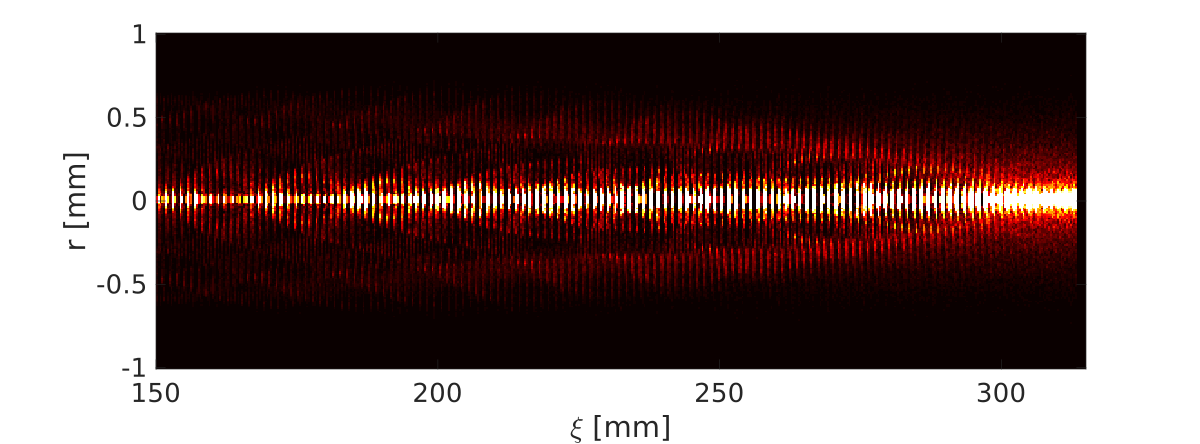
\includegraphics[width=1.0\linewidth]{figures/PBSelfModulation}
    \caption{\label{Fig:Sim:SMI} An example of a seeded SPS proton beam having undergone self-modulation in about $3\unit{m}$ of plasma. The halo of protons ejected from the defocusing regions can be clearly seen, leaving a core of micro bunches on the beam axis.}
\end{figure}

\todo[inline]{Add plot of initial proton beam.}

% ================================================================================================================================ %

\subsection{With a Pre-Modulated Beam}
\label{Sim:PBPreMod}

The half SPS proton beam is about $30\unit{cm}$ long.
In order to make the simulations more manageable in size for the beam loading studies, we decided to move to a sample proton beam of 26 micro bunches -- an order of magnitude smaller than the previous case.

These simulations were all done using OSIRIS 3.0.
With this version it is necessary for the beams to drift in vacuum for a short distance for the electro-magnetic fields to develop properly, as they are initialised at zero (see further discussion in Section~\ref{PIC:Full}).
Since the evolution of the self-modulation instability was not of primary interest at this stage, we chose to modify the beam profile to emulate a section of the modulated bunch.
We refer to this as \textit{pre-modulation}.
This was done by shortening the period of the density envelope cosine function from Equation~\ref{EQ:SPS-Profile} to match that of the plasma wavelength.
\begin{equation}
    f(\xi,r) = A\sqrt{2} \left[\frac{1}{2\sqrt{2}}
             + \cos\left(k_{pe}\xi - \mu\right)\right] \exp\left(-\frac{r^{2}}{2\sigma_{r}^{2}}\right), \label{EQ:PB-PreMod}
\end{equation}
where $\mu$ is the position of the first micro bunch, and $k_{pe}$ is the plasma wave number~\cite{berglyd_olsen:2015}.
The offset of the cosine function is chosen such that the width of the micro bunch matches the width of a bunch in the simulations done with a full bunch, and there is a gap between the bunches that approximates the gaps we see between micro bunches in the simulated self-modulated case.
Since OSIRIS ignores profile densities with negative values, the profile is automatically clipped at $0$, requiring no further manipulation of the profile function to remove negative values.

Again, cosines are preferred over a series of Gaussian bunch profiles, although this time because the cosine is periodic, and because OSIRIS' mathematical functions cannot be longer than 256 characters.

Generating an equidistant bunch train in this manner causes the head of the second bunch to be partially defocused causing a decay of the micro bunches by the wakefield of the first bunch.
This effect was not directly compensated for in Publication~\ref{Pub:IPAC15}.
This can be avoided by increasing the separation between the first and second bunch from $2\pi c/\omega_p$ to $(2\pi+\pi/4) c/\omega_p$~\cite{lotov:2018}.

The charge of the proton micro-bunches were matched to that of a micro-bunch generated by the self-modulation instability in the initial simulations.
This charge density decreases towards the back end of the modulated beam, so they were fixed to a charge for the region were the injection of an electron bunch is reasonable.
For the pre-modulated simulations, this number was set to $100\unit{pC}$ such that the total charge of the sample proton beam was $2.6\unit{nC}$.
This corresponds to a peak current of $135\unit{A}$.
The electron witness bunch was injected between bunch 20 and 21.

\todo[inline]{Include the standard pre-modulation plots used in several presentations.}

% ================================================================================================================================ %

\subsection{With a Single Drive Bunch}
\label{Sim:PBSingle}

Further approximations needed to be made to decrease the scale of the problem in order to study the beam loading and evolution of the electron witness beam more directly.
Even the pre-modulated proton beam is somewhat costly to simulate -- both because it still requires a multiple plasma-wavelength simulation box length, and because a large number of simulated particles are needed to populate the beam profile.
These proved to be a challenge when doing larger parameter scans as the CPU cost would rise to levels beyond available resources.
While additional resources could potentially have been requested, we considered the option to exclude the evolution of the proton beam entirely from our studies and instead assume the region where the electron bunch was injected to have the properties laid out in the AWAKE status reports~\cite{awake_collaboration:2016}.
%add explicit description, charge, wakefield.

In the single bunch studies we therefore approximated the proton drive beam ahead of the witness bunch injection region as a single, ideal proton drive bunch generating the expected wakefields.
To reproduce these conditions, we used a Gaussian bunch of $1.46\nexp{10}$ protons corresponding to $2.34\unit{nC}$, a length $\sigma_{z} = 40\unit{\mu m}$ corresponding to $7\unit{kA}$, and a transverse size $\sigma_{x,y}=200\unit{\mu m}$~\cite{berglyd_olsen:2018}.

\todo[inline]{Include a plot of the single bunch as well.}

% ================================================================================================================================ %
\section{Simulating the Witness Bunch}
\label{Sim:EBeam}

\todo[inline]{This section needs to be completed.}
There were a few points to consider when simulating the electron witness beam.
They differ between the two simulation codes used in these studies.

% ================================================================================================================================ %
\subsection{Witness Bunch Size and Resolution}
\label{Sim:EBeam:SizeRes}

For the early simulations, a transverse size of $\sigma_{x,y}=105\unit{\mu m}$ was used, see Table~\ref{T:AWAKERuns}.
For later simulations, when the beam transverse size was matched to its emittance and the plasma density (see Section~\ref{Int:BPI:Match}), much narrower beams were used -- on the order of a few micrometres.
The proton drive beam size is tied to the plasma skin depth (see Section~\ref{Int:DBeam:SMI}), which is $200\unit{\mu m}$.
This, naturally, poses a resolution challenge when very narrow electron beams need to be resolved, while at the same time, the simulation box needs to also be able to contain the proton drive bunch.

For the simulations with a pre-modulated proton beam, used for Publication~\ref{Pub:IPAC15}, the simulation box had a radius of $2.12\unit{mm}$ with $425$ grid cells, resulting in a resolution of $5\unit{\mu m}$.
This is more than sufficient to resolve and contain both the beams, with a small buffer for the plasma (see Section~\ref{Sim:Plasma}).
For the single drive bunch studies, Publications~\ref{Pub:NAPAC16} and~\ref{Pub:BL17}, the transverse grid resolution had to be increased.
In most cases we tried to resolve the witness bunch with at least $5$ grid cells per $\sigma_{x,y}$, although this was in some instances increased.
It was also important to keep an eye on the distribution of macro particles on the simulation grid.
This was especially important for the OSIRIS 3.0 based simulations, as OSIRIS creates macro particles of varying charge, with a fixed number of particles per cell defined by input parameters.
Since most OSIRIS simulations were run with a 2D cylindrical geometry, the $1/r$ factor enters into the electromagnetic field equations.
This results in numerical noise when $r \to 0$, which in return affects the evolution of the bunch itself.
A sample of the 2D cylindrical simulations were re-run with 3D Cartesian coordinates in order to check that the results were not dominated by this noise.

QuickPIC uses 3D Cartesian coordinates, and thus does not have the $1/r$ problem.
In addition, it has a fixed charge per beam macro particle, and instead varies the number of these per grid cell to create a charge distribution.
A convergence scan of resolution dependency was performed for Publication~\ref{Pub:BL17} to check that the results did not depend on resolution within the range we used for this study. The convergence scan is described in Section~\ref{SimA:Converge}.
QuickPIC defines resolution in exponents of $2$, and thus are locked to a set of values that rapidly increase for each step.
The simulations used for Publication~\ref{Pub:BL17} were done with transverse grids of $2^{9}$ and $2^{10}$ ($512 \times 512$ and $1024 \times 1024$) cells, resolving a box size of $1.2\unit{mm}$ square.
In the former case, the grid cell size was thus as large as $2\unit{\mu m}$ for the former case, and $1\unit{\mu m}$ for the latter.
This did, however, not appear to have any significant impact on the results.

Further details on how QuickPIC and OSIRIS handle beam particles is covered in Appendix~\ref{Apx:PIC}.

% ================================================================================================================================ %
\subsection{Witness Bunch Transverse Evolution}
\label{Sim:EBeam:TEvol}

In OSIRIS 3.0, the electromagnetic fields are initialised at zero.
It is therefore necessary to let the beams drift a short distance before they enter the plasma region, in order for the fields to develop.
Due to this initial drift stage, it was technically challenging to inject an electron witness bunch while strictly controlling parameters like emittance, energy spread and transverse size as during the drift phase, these parameters undergo evolution.
There are, however, possible to prevent the beam from evolving by slowly ramping up the beam charge or the beam energy.
During these ramping stages, the macro particles are prevented from transverse evolution.

For the early studies, and for Publication~\ref{Pub:IPAC15}, only beam loading and acceleration was considered, but for Publications~\ref{Pub:NAPAC16} and \ref{Pub:BL17}, it was necessary to control the witness bunch emittance.
While QuickPIC has input parameters defining beam emittance in each direction, OSIRIS 3.0 does not.
OSIRIS 3.0 does, however, let one define spatial and momentum distributions independently (see Appendix~\ref{Apx:PIC}).
However, as correlation between $\sigma_{p_{i}}$ and $\sigma_{i}$, for dimension $i$, cannot be controlled, the beam can only be initialised at waist (Twiss parameter $\alpha = 0$, see Appendix~\ref{Apx:DA}).

For the OSIRIS simulations, the ramping parameters were tuned such that the bunch was unfrozen a few micrometres before it entered the plasma.
This prevented betatron oscillations, ensuring that the bunch was still at waist when it entered the plasma region.

% ================================================================================================================================ %
\section{Simulating the Plasma}
\label{Sim:Plasma}

For the simulations made with OSIRIS 3.0, where an initial drift stage is necessary, a decision had to be made on how to simulate the entry point into the plasma.
Early tests showed that freezing the transverse evolution of the electron beam and releasing it immediately before the entry into plasma, posed a few challenges.
The sudden change in conditions is itself unphysical, and the abrupt change from a frozen state to an evolving bunch while at the same time seeing an instant step in plasma density from $0$ to $7\nexp{14}\unit{cm}^{-3}$, made it challenging to interpret the results.
This was especially the case when the witness bunch was not matched to the plasma density (see Section~\ref{Int:BPI:Match}).
A rapid pinching of the bunch occurred immediately after entering the plasma region, causing a spike in the charge density that was within a region too narrow to resolve with the grid resolution we used.
This is also a numerically noisy region, as discussed in Section~\ref{Sim:EBeam:SizeRes}.
Eliminating the hard plasma edge by introducing a more realistic plasma ramp over $10\unit{mm}$, using a cosine-shaped density function. was attempted.
However, the effect on the witness bunch was not significant.

% ================================================================================================================================ %
% \subsection{Plasma Gradient}
% \label{Sim:Plasma:Grad}

% Examples from IPAC15 on gradient versus erosion. Maybe cite Alexey et al?

    %
%  Simulations
% =============
%

\chapter{Simulation Analysis}
\label{Ch:SimA}

This chapter outlines some of the key considerations and calculations performed on the data sets generated in these simulations.
Analysis tools were developed in MATLAB for both OSIRIS and QuickPIC data sets.
These are available online, and are described in more detail in Appendix~\ref{Apx:DA}.

% ================================================================================================================================ %
\section{Extracting Twiss Parameters from Particle Arrays}
\label{SimA:EnTwiss}

Both OSIRIS and QuickPIC dump the macro particles as large arrays of six-dimensional data, providing each particle's position and momentum vector.
QuickPIC uses equally weighted macro particles, greatly simplifying the analysis.
OSIRIS, however, uses weighted macro particles, so the weights need to be considered when performing the statistical calculations.
Additional statistical functions were added to MATLAB's own to perform these weighted calculations (see Appendix~\ref{Apx:DA}).

To study the collective motion of particles it is useful to calculate the bunch total emittance in terms of the RMS value or standard deviation of its particles.
Equation~\ref{EQ:EmittFull} from Section~\ref{Int:BPI:EnTwiss} can be rewritten in terms of the statistical distributions of its particles such that
\begin{equation}
    \epsilon = \sqrt{\gamma\sigma_{x}^{2} + 2\alpha\sigma_{x}\sigma_{x^{\prime}} + \beta\sigma_{x^{\prime}}^{2}}, \label{EQ:Emitt}
\end{equation}
where the angle of the $i$-th particles can be taken from its momentum
\begin{equation}
    x_{i}^{\prime} = \frac{p_{i,x}}{p_{i,z}}.
\end{equation}

For a set of macro particles, the geometric emittance can be calculated directly by taking the covariance matrix of the $x$ and $x^{\prime}$ vectors
\begin{equation}
    \mathbf{T} = \mathrm{cov}\left(\mathbf{x}, \mathbf{x}^{\prime}\right), \label{EQ:ECalc1}
\end{equation}
and then taking the square root of its determinant
\begin{equation}
    \epsilon = \sqrt{\mathrm{det}\left(\mathbf{T}\right)}. \label{EQ:ECalc2}
\end{equation}
The Twiss parameters can be extracted from the matrix $\mathbf{T}$ as well:
\begin{equation}
    \alpha = \mathrm{T}_{12}/\epsilon, \quad
    \beta  = \mathrm{T}_{11}/\epsilon, \quad
    \gamma = \mathrm{T}_{22}/\epsilon.
\end{equation}

% ================================================================================================================================ %
\section{A Measure for Beam Quality}
\label{SimA:QTilde}

For the emittance study in Publication~\ref{Pub:BL17} it was necessary to define a convenient unit for the quality of the accelerated bunch in terms of emittance evolution in regions along the bunch length.
In the quasi-linear plus non-linear regime this publication investigates, emittance growth only occurs at the head of the bunch.
However, the region of emittance growth varies when parameters such as charge and beam size changes.
In the study we defined a parameter that quantifies emittance preservation,
\begin{equation}
    \tilde{Q} = \frac{1}{N} \sum_{m=0}^{M} \sum_{n=0}^{N} Q_{m+n}\,\chi(\xi_{m},N),\label{EQ:BeamQ}
\end{equation}
where $M$ is the number of longitudinal grid slices of length $\Delta\xi$ which contains macro particles for the witness bunch, and with corresponding coordinate $\xi_{m}$.
$N$ is the number of such slices to average over.
And $\chi(\xi_{m},N)$ is the step function
\begin{equation}
    \chi(\xi_{i},N) =
    \begin{cases}
        1, & \frac{\epsilon_{i} - \epsilon_{0}}{\epsilon_{0}} \leq 5\% \\
        0, & \frac{\epsilon_{i} - \epsilon_{0}}{\epsilon_{0}} > 5\%
    \end{cases}
    \quad\mathrm{for~}\epsilon_{i}\mathrm{~over~the~interval}\quad
    [\xi_{i}, \xi_{i} + N\Delta\xi],
\end{equation}
where $\epsilon_{i}$ is the emittance as defined by Equations~\ref{EQ:ECalc1} and~\ref{EQ:ECalc2} for a set of macro particles within the interval $\xi_{i}$ to $\xi_{i} + N\Delta\xi$, and $\epsilon_{0}$ is the initial emittance defined in the simulation input file.
For the studies included in Publication~\ref{Pub:BL17},
\begin{equation}
    M = \left\lfloor \frac{10\sigma_{z}}{\Delta\xi} \right\rceil, \quad
    N = 4.
\end{equation}
The first slice coordinate for the iterator $m$ is
\begin{equation}
    \xi_{m=0} = \mu_{\mathrm{eb}} - 5\sigma_{z,\mathrm{eb}} - 0.5\Delta\xi,
\end{equation}
where $\mu_{\mathrm{eb}}$ is the longitudinal centre of the bunch.

The quantity $\tilde{Q}$ is thus the total charge that retains its initial emittance within a limit of $5\%$ growth.
The emittance is calculated with a moving window of $4$ grid cells over $\pm 5\sigma_z$ of the bunch.

\paragraph{Note:} This method may yield a misleading result if the Twiss parameter $\alpha$ varies too much along the length of the bunch.
That is, a rotation of the phase-space ellipse, see Figure~\ref{Fig:BPI:Twiss}.
The emittance can be locally small and qualify for the $5\%$ criterion, even if the total emittance of the region included in $\tilde{Q}$ is not.
This can easily be checked after the seemingly optimal region of the bunch is known by verifying that its total emittance does not exceed the same criterion.

% ================================================================================================================================ %
%  Full Scale Studies
% ================================================================================================================================ %
\section{Full Scale Studies}
\label{SimA:FullScale}

A total of 38 simulations of a full AWAKE proton bunch, with and without an injected electron bunch, were run.
As can be seen from Table~\ref{T:SimCost}, these simulations took an average of over $11\,000$ CPU hours each.
The simulation parameters used for these studies are described in Section~\ref{Sim:PBeam}.

The purpose of the full scale studies were mainly to develop some familiarity with OSIRIS~3.0, but also to study the properties of the self-modulated beam in order to make a reasonable approximation of it for the later pre-modulated studies (see Section~\ref{Sim:PBPreMod}).

The modulation period of the self-modulated beam was checked with Fast Fourier Transform (FFT)~\cite{van_loan:1992}.
The FFT revealed that the core modulation frequency is indeed the characteristic frequency of the plasma as presented in Publication~\ref{Pub:IPAC15}.

\begin{figure}[hbt]
    \centering
    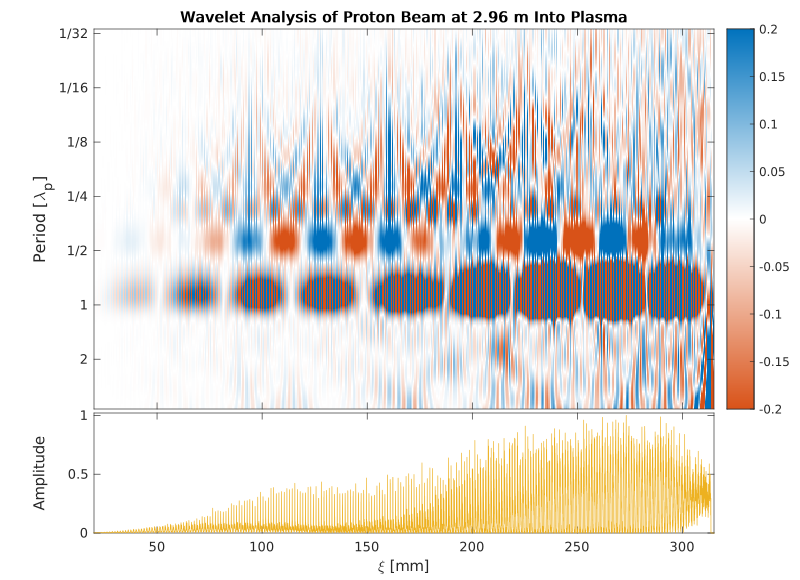
\includegraphics[width=1.0\linewidth]{figures/PBSMIWavelet}
    \caption{\label{Fig:SimA:Wavelet}
        A wavelet analysis of the beam shown in Figure~\ref{Fig:Sim:SMI}, at the same position in the plasma, using Morlet wavelet analysis~\cite{torrence:1998}.
        The horizontal axis shows the position~$\xi$ in the simulation box.
        The vertical axis shows the Fourier period in units of the plasma wavelength~$\lambda_p$.
        This density plot is the absolute value of the complex wavelet data, showing clearly the peak in frequency in the area around the plasma wavelength.
        The colour axis is saturated at amplitude $1$ in order to show the fine structure of the harmonics.
        The contour plot overlay shows the full range of the density data in steps of $0.5$.
    }
\end{figure}

A wavelet analysis was also performed using a Morlet wavelet analysis~\cite{goupillaud:1984,bernardino:2005}.
The wavelet adds some additional information about the modulation frequency as a function of position along the modulated beam of micro bunches.
Such a plot is shown in Figure~\ref{Fig:SimA:Wavelet} where the proton bunch has propagated through about $3\unit{m}$ of plasma.
The figure shows the magnitude of the wavelet analysis data~\cite{lee:1994}, and the amplitude indicates that the density variation is the highest at the front of the bunch (compare with initial profile in Figure~\ref{Fig:Sim:SMI}).

The frequency of the pre-modulated beam was slightly adjusted such that the FFT profiles matched that of the full scale SMI simulations~\cite{berglyd_olsen:2015}.

Both FFT and Wavelet analysis tools were implemented in the \textit{OsirisAnalysis} package described in Section~\ref{Tools:OAAdd}.

% ================================================================================================================================ %
%  Beam Loading and Energy Spread
% ================================================================================================================================ %
\section{Beam Loading and Energy Spread}
\label{SimA:BLoad}

When the parameters of the self-modulated bunch had been established, and the pre-modulated studies set up as laid out in Section~\ref{Sim:PBPreMod}, the evolution of the electron bunch became the main focus.
Of particular interest in the early studies was the beam loading of the electron witness bunch on the longitudinal wakefields, as well as its energy spread as it propagated through the plasma section.

The transverse size of the bunch was initially chosen to be $\sigma_{x,y}=105\unit{\mu m}$, see Table~\ref{T:AWAKERuns}.
This is the size initially proposed for Run~1.
The longitudinal size was chosen to be $\sigma_{z}=40\unit{\mu m}$ for the studies included in Publication~\ref{Pub:IPAC15}, but several lengths were tested in simulations.

\begin{figure}[hbt]
    \centering
    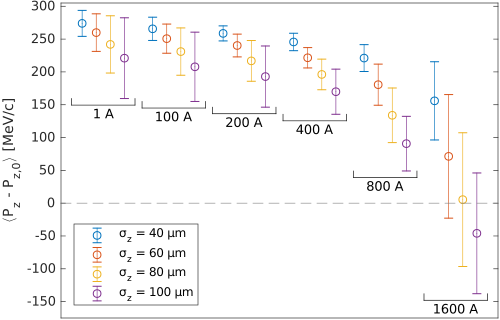
\includegraphics[width=0.625\linewidth]{figures/NAPACEGainSpreadScan}
    \caption{\label{Fig:SimA:BLoadScan}
        A parameter scan for the 26 bunch pre-modulated studies where six different bunch currents and four different bunch lengths were considered.
        The energy gain $P_{z} - P_{z,0}$ after $1.1\unit{m}$ of plasma is shown with the error bars representing the RMS energy spread.
        The figure is presented in Publication~\ref{Pub:NAPAC16} and in Adli \etal~\cite{adli:2016a}.
    }
\end{figure}

Tuning the longitudinal size is essential.
On the one hand, a short bunch positioned at an optimal accelerating phase ensures a low energy spread as all electrons see close to the same accelerating field.
On the other hand, a long bunch is capable of holding a larger charge without the charge density becoming critical.
The bunch length and charge the field is able to support can be improved by tuning the parameters such that the field is flat in the region where the witness bunch is located, as discussed in Section~\ref{Int:BPI:BLoad}.

The initial studies showed that $\sigma_{z} = 40-60\unit{\mu m}$ is a good compromise between having a short enough bunch to stay within the accelerating region of the accelerating wakefield, $\approx \lambda_{pe}/4$ (see Section~\ref{Int:BPI:BLoad}), and a long enough bunch to contain a reasonable amount of electrons without overloading the wakefield.
A larger parameter scan was performed for Publication~\ref{Pub:NAPAC16}, and was presented as a contributing talk at North American Particle Accelerator Conference in Chicago in 2016.
It was also included in~\cite{adli:2016a}.
The main results of this parameter scan is shown in Figure~\ref{Fig:SimA:BLoadScan}.

% ================================================================================================================================ %
%  Emittance Evolution
% ================================================================================================================================ %
\section{Emittance Evolution}
\label{SimA:Emitt}

Achieving a large energy gradient and a low energy spread while maximising charge is a compromise between parameters~\cite{berglyd_olsen:2018}.
High charge density affects beam loading which, when mismatched, may lead to increased energy spread.
An overloaded accelerating field will also reduce energy gain through the accelerating region.
In addition to these considerations, we also seek to preserve the initial emittance and avoid emittance growth.

\begin{figure}[hbt]
    \centering
    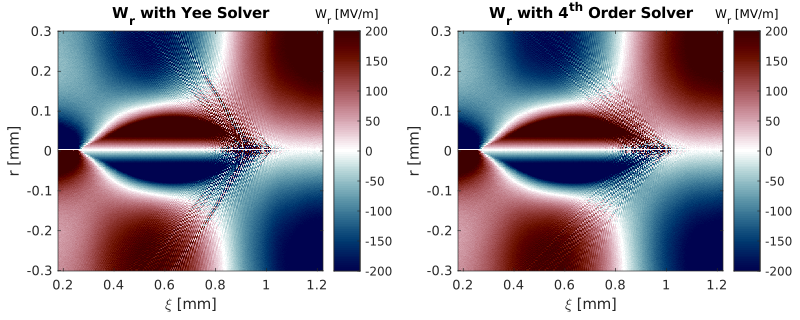
\includegraphics[width=0.999\linewidth]{figures/EMFSolverNoise}
    \caption{\label{Fig:SimA:EMFNoise}
        The radial wakefields $W_r$ for two test simulations of a high density electron bunch.
        The numerical noise generated by the electromagnetic field solvers is clearly seen as additional short period ``wake ripples''.
        The data is taken at the entry into the plasma region, and shows results for both the Yee solver and the slightly better 4\ts{th} order solver in OSIRIS 3.0.
        Both simulations were run without smoothing.
        Tests with smoothing of the fields had some effect.
        The colour axis is truncated to show the structure of the noise.
        The peak of the noise is $3-4$ times higher.
    }
\end{figure}

The simulations for Publication~\ref{Pub:NAPAC16} did not focus on emittance, and were therefore run with OSIRIS~3.0, which is a full PIC code (see Appendix~\ref{Apx:PIC}).
However, due to the numerical noise in the electromagnetic field solver associated with full PIC codes, as also discussed in the appendix, we opted to use QuickPIC at this stage.
Before we moved to QuickPIC, we ran a number of test simulations probing the scale of the noise issue.
OSIRIS provides a number of solvers and filters to minimise the issue, but as illustrated in Figure~\ref{Fig:SimA:EMFNoise}, it was too large of an issue for our specific case with a high density electron bunch.

% ================================================================================================================================ %
\subsection{The Quasi-Linear Regime}
\label{SimA:QLin}

As AWAKE operates in the quasi-linear regime, all the simulations were run with a plasma density matching the expected conditions in the experiment's vapour cell for Run~2.
The quasi-linear regime has the benefit of combining near radially uniform accelerating fields with a nearly non-linear wake (see Section~\ref{Int:BPI:QLin}).

\begin{figure}[hbt]
    \centering
    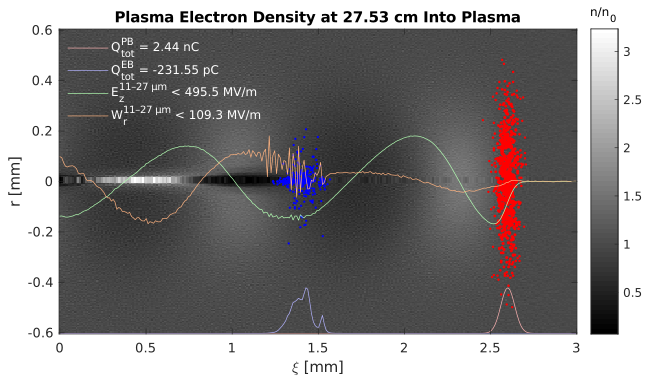
\includegraphics[width=0.8125\linewidth]{figures/NAPACPlasmaDensity}
    \caption{\label{Fig:SimA:NAPACPD}
        Loading of the field after for a $500\unit{A}/60\unit{\mu m}$ electron bunch.
        A sample of electrons can be seen in blue, and protons in red, as well as their respective projections at the bottom.
        The $E_z$ and $W_r$ wakefields are also shown in green and brown respectively.
        The figure is recreated from Publication~\ref{Pub:NAPAC16}.
    }
\end{figure}

However, in the presence of a high density electron witness bunch, a secondary bubble forms behind it.
This bubble is typically non-linear.
The simulations for Publication~\ref{Pub:NAPAC16} showed that this was the case for our optimal range of bunch size and density.
One such example is shown in Figure~\ref{Fig:SimA:NAPACPD}, taken from Publication~\ref{Pub:NAPAC16}.
We labelled this setup as the \textit{Quasi-Linear + Non-Linear Case}.

% ================================================================================================================================ %
\subsection{The Quasi-Linear + Non-Linear Case}
\label{SimA:QLinNonLin}

An electron witness bunch matched to the typical AWAKE plasma density will be, as discussed in Section~\ref{Int:BPI:Match}, very narrow.
At a typical normalised emittance of $2.0\unit{\mu m}$, the matched bunch $\sigma_r$ is $5.25\unit{\mu m}$.
Even at low charge and at the upper limit in terms of bunch length, the wakefields of such a bunch will quickly reach the non-linear regime.
In the base case used in the beam loading study in Publication~\ref{Pub:BL17}, the peak density of the bunch $n_b/n_0 > 35$, is well beyond the saturation level of the bubble that occurs when $n_b/n_0 > 10$ \cite{lu:2005}.

\begin{figure}[hbt]
    \centering
    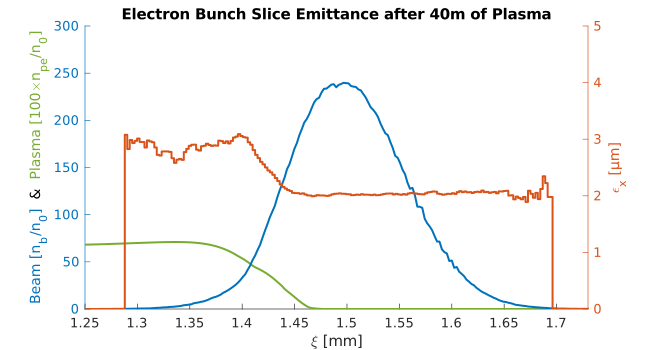
\includegraphics[width=0.8125\linewidth]{figures/40mSliceEmittance}
    \caption{\label{Fig:SimA:BL17Emitt}
        Emittance of an electron bunch along the $\xi$ axis.
        The emittance of the slices are computed with a moving average window of four grid cells or $\approx 9.4\unit{\mu m}$, and shown in red.
        The corresponding electron witness bunch density is shown in blue and the plasma electron density in green.
        The bunch is shown after having propagated through $40\unit{m}$ of plasma.
        The initial emittance for this simulation was $2\unit{\mu m}$, and there is no significant emittance growth in the region in the bunch's own bubble.
        The bunch travels towards the left of the figure.
    }
\end{figure}

The implication here is that there is an additional beneficial effect of loading the accelerating field with as much charge as it will allow without overloading it.
The resulting non-linear wake driven by the head of the bunch, which will see emittance growth due to the quasi-linear conditions of the proton wake, ensures that the rest of the bunch sees a strong focusing force from the pure ion column preventing further emittance growth.
As the electron bunch gains energy, its transverse size will decrease as its emittance is preserved as $\sigma_{r} = \sqrt{\emitN\beta}$~\cite{wille:2001}.
This is clearly shown in Figure~\ref{Fig:SimA:BL17Emitt}, generated from the same data as presented in Publication~\ref{Pub:BL17}.
The head of the bunch sees an emittance growth to about $3\unit{\mu m}$, while the bulk of the bunch sees none.

With this setup there is a range of parameters that needs fine tuning.
In Publication~\ref{Pub:BL17}, we performed a number of parameter scans, attempting to maximise beam quality as defined in Equation~\ref{EQ:BeamQ}.

% ================================================================================================================================ %
\subsection{Convergence Scan}
\label{SimA:Converge}

For the large parameter scans performed for Publication~\ref{Pub:BL17}, it was necessary to verify that the results were not dependant on grid resolution.
The radial wakefields within the plasma bubble are linear, but so are the fields within one grid cell as they are interpolated on the grid.
The effect of linear focusing could thus be an artefact of resolution.
That is especially true in the case where the grid cells were only a factor $2.5$ smaller than the bunch $\sigma_{x,y}$, and thus the bubble radius also small.

\begin{table}[hbt]
    \centering
    \caption{Convergence results for a reference simulations for Publication~\ref{Pub:BL17}.
    The reference bunch has a charge of $250\unit{pC}$, and the emittance tolerance criterion for the $\tilde{Q}$ parameter is $5\%$ (see Section~\ref{SimA:QTilde}).}
    \label{T:Converg}
    \begin{tabularx}{132mm}{Xl d{1}l d{1}l d{1}l}
        \rowcolor{tblhead}
        \texthh{Length} & \texthh{Param.}
            & \multicolumn{2}{c}{\texthh{1024$\times$1024}}
            & \multicolumn{2}{c}{\texthh{2048$\times$2048}}
            & \multicolumn{2}{c}{\texthh{4096$\times$4096}} \\
        \hline
                         & $\tilde{Q}$ &  213.9 & $\unit{pC}$  &  206.9 & $\unit{pC}$  &  213.1 & $\unit{pC}$  \\
        $40\unit{\mu m}$ & MEAN$(E)$   & 2263   & $\unit{MeV}$ & 2233   & $\unit{MeV}$ & 2247   & $\unit{MeV}$ \\
                         & STD$(E)$    &  267.4 & $\unit{MeV}$ &  250.4 & $\unit{MeV}$ &  261.5 & $\unit{MeV}$ \\
        \hline
                         & $\tilde{Q}$ &  221.6 & $\unit{pC}$  &  222.0 & $\unit{pC}$  &  222.1 & $\unit{pC}$  \\
        $60\unit{\mu m}$ & MEAN$(E)$   & 2346   & $\unit{MeV}$ & 2336   & $\unit{MeV}$ & 2333   & $\unit{MeV}$ \\
                         & STD$(E)$    &  166.8 & $\unit{MeV}$ &  165.0 & $\unit{MeV}$ &  165.5 & $\unit{MeV}$ \\
        \hline
                         & $\tilde{Q}$ &  229.9 & $\unit{pC}$  &  226.9 & $\unit{pC}$  &  224.8 & $\unit{pC}$  \\
        $80\unit{\mu m}$ & MEAN$(E)$   & 2378   & $\unit{MeV}$ & 2379   & $\unit{MeV}$ & 2368   & $\unit{MeV}$ \\
                         & STD$(E)$    &  120.0 & $\unit{MeV}$ &  117.6 & $\unit{MeV}$ &  119.1 & $\unit{MeV}$ \\
    \end{tabularx}
\end{table}

% ================================================================================================================================ %
\section{Summary of Simulation Studies}
\label{SimA:Summary}

Table~\ref{T:SimCost} gives an overview of the simulation studies done as a part of the thesis work.
Nearly all of the 1.5 million CPU hours used for these simulations were done using the super computer \textit{Abel}, located at the the USIT department at the University of Oslo and owned by the University of Oslo and The Norwegian Metacenter for Computational Science.
Project code for the computing access was \texttt{nn9303k}.

Some of the simulations were also run on the computing cluster \textit{Smaug} hosted at the Department of Physics and maintained by the students at Computational Physics.

\begin{table}[hbt]
    \centering
    \caption{Overview of total simulation cost. $97\%$ of the simulations were run on the supercomputer \textit{Abel}, on Oct Core Intel Xeon E5-2670 CPUs. The remainder were run on older nodes with Quad Core AMD Opteron 2354 CPUs.}
    \label{T:SimCost}
    \begin{tabularx}{\textwidth}{Xlrrr}
        \rowcolor{tblhead}
        \texthh{Topic of Studies}                & \texthh{Code} & \texthh{Count} &     \texthh{CPU Time} &  \texthh{Average} \\
        \hline
        Preliminary studies (mostly testing)     & OSIRIS        &           $21$ &    $266\,599\unit{h}$ & $12\,695\unit{h}$ \\
        Full length AWAKE proton bunch studies   & OSIRIS        &           $38$ &    $440\,583\unit{h}$ & $11\,594\unit{h}$ \\
        Pre-modulated beam studies$^{1}$         & OSIRIS        &          $144$ &    $319\,093\unit{h}$ &  $2\,216\unit{h}$ \\
        3D reference studies                     & OSIRIS        &           $23$ &    $245\,974\unit{h}$ & $10\,695\unit{h}$ \\
        Single drive bunch studies$^{2}$         & OSIRIS        &          $124$ &     $47\,837\unit{h}$ &     $386\unit{h}$ \\
        Beam loading and emittance studies$^{3}$ & QuickPIC      &          $293$ &    $369\,887\unit{h}$ &  $1\,262\unit{h}$ \\
        \hline
        \rowcolor{tblfoot}
        Total                                    &               &          $657$ & $1\,479\,350\unit{h}$ &  $2\,252\unit{h}$ \\
        \multicolumn{5}{p{50mm}}{\footnotesize
            $^{1}$ Main studies for Publication \ref{Pub:IPAC15} \newline
            $^{2}$ Main studies for Publication \ref{Pub:NAPAC16} \newline
            $^{3}$ Main studies for Publication \ref{Pub:BL17} \newline
        }
    \end{tabularx}
\end{table}

% ================================================================================================================================ %

    %
%  Summary and Conclusion
% ========================
%

\chapter{Summary and Conclusion}
\label{Ch:SnC}

Text



% Formatting for Appendices and Publications
\titleformat{\chapter}[display]%
    {\Large\sffamily\scshape}%
    {\textcolor{appendix}\chaptertitlename\ \textcolor{appendix}\thechapter}%
    {2mm}%
    {\Huge\sffamily\upshape}

\addtocontents{toc}{\cftpagenumbersoff{part}}

% Publications

\cleardoublepage
\bookmarksetup{startatroot}
\phantomsection
\part*{Publications}
\label{A:Pub}

\pagestyle{plain}
\renewcommand{\appendixtocname}{Publications}
\renewcommand{\appendixname}{Publication}

\appendix
    \setcounter{chapter}{0}
    \renewcommand{\thechapter}{\Roman{chapter}}
    \renewcommand{\theHchapter}{\Roman{chapter}}
    %
%  Publication 1 :: IPAC 2015
% ============================
%

\chapter{Loading of a Plasma-Wakefield Accelerator Section\\Driven by a Self-Modulated Proton Bunch}
\label{Pub:IPAC15}

\begin{hangparas}{10mm}{1}

    \textbf{Abstract:}
    Abstract

    \vspace{8mm}

    \textbf{Authors:}
    V. K. Berglyd Olsen, E. Adli (University of Oslo, Oslo, Norway)
    P. Muggli (Max Planck Institute for Physics, Munich, Germany and CERN, Geneva, Switzerland)
    J. M. Vieira (Instituto Superior Technico, Lisbon, Portugal)


    \vspace{5mm}

    \textbf{Publication:}
    Proceedings of IPAC 2015, Richmond, Virginia, USA

    \vspace{5mm}

    \textbf{Date:}

\end{hangparas}

    \cleardoublepage
    \includepdf[pages=1-last,scale=0.95,pagecommand={}]{files/IPAC15-WEPWA026.pdf}
    %
%  Publication 2 :: NAPAC 2016
% =============================
%

\chapter[Loading of Wakefields in a Plasma Accelerator Section Driven by a Self-Modulated\\Proton Beam,%
        ~\textit{Proceedings of NAPAC 2016}]%
        {\Large Loading of Wakefields in a Plasma Accelerator Section\\Driven by a Self-Modulated Proton Beam}
\label{Pub:NAPAC16}

\begin{description}

    \item[Abstract:]
    Using parameters from the AWAKE project and particle-in-cell simulations we investigate beam loading of a plasma
    wake driven by a self-modulated proton beam. Addressing the case of injection of an electron witness bunch after
    the drive beam has already experienced self-modulation in a previous plasma, we optimise witness bunch parameters of
    size, charge and injection phase to maximise energy gain and minimise relative energy spread and emittance of the
    accelerated bunch.

    \item[Authors:]
    Veronica K. Berglyd Olsen, Erik Adli (University of Oslo, Oslo, Norway),
    Patric Muggli (Max Planck Institute for Physics, Munich, Germany and CERN, Geneva, Switzerland),
    Jorge M. Vieira (Instituto Superior Technico, Lisbon, Portugal)

    \item[Publication:]
    Proceedings of NAPAC 2016, Chicago, Illinois, USA \cite{berglyd_olsen:2016}

    \item[Date:]
    9\ts{th} to 14\ts{th} of October, 2016

\end{description}

    \cleardoublepage
    \includepdf[pages=1-last,scale=0.95,pagecommand={}]{files/NAPAC16-TUA4CO03.pdf}
    %
%  Publication 4 :: IPAC 2017
% ============================
%

\chapter{Data Acquisition and Controls Integration of the AWAKE Experiment at CERN}
\label{Pub:IPAC17}

\begin{hangparas}{10mm}{1}

    \textbf{Abstract:}
    The AWAKE experiment has been successfully installed in the CNGS facility at CERN, and is
    currently in its first stage of operation. The experiment seeks to demonstrate self-modulation
    of an SPS proton beam in a rubidium plasma, driving a wakefield of several gigavolt per meter.
    We describe the data acquisition and controls system of the AWAKE experiment, its integration
    into the CERN controls system and new control developments specifically required for the AWAKE
    experiment.

    \vspace{8mm}

    \textbf{Authors:}
    Veronica K. Berglyd Olsen (University of Oslo, Oslo),
    Edda Gschwendtner (CERN, Geneva),
    Spencer Jake Gessner (SLAC, Menlo Park, California)

    \vspace{5mm}

    \textbf{Publication:}
    Proceedings of IPAC 2017, Copenhagen, Denmark

    \vspace{5mm}

    \textbf{Date:}

\end{hangparas}

    \cleardoublepage
    \includepdf[pages=1-last,scale=0.95,pagecommand={}]{files/IPAC17-TUPIK061.pdf}
    %
%  Publication 3 :: Peer Review
% ==============================
%

\chapter{Placeholder Title}
\label{Pub:PRev17}

\begin{hangparas}{10mm}{1}

    \textbf{Abstract:}
    Abstract

    \vspace{8mm}

    \textbf{Authors:}
    Veronica K. Berglyd Olsen (University of Oslo, Oslo)

    \vspace{5mm}

    \textbf{Publication:}
    Journal

    \vspace{5mm}

    \textbf{Date:}

\end{hangparas}

    \cleardoublepage
    \includepdf[pages=1-last,scale=0.95,pagecommand={}]{files/BeamLoading17.pdf}

% Appendices

\cleardoublepage
\bookmarksetup{startatroot}
\phantomsection
\part*{Appendices}
\label{A:App}

\pagestyle{fancy}
\renewcommand{\appendixtocname}{Appendices}
\renewcommand{\appendixname}{Appendix}
\renewcommand{\headrulewidth}{0.5pt}
\defaulthead

\appendix
    \setcounter{chapter}{0}
    \renewcommand{\thechapter}{\Alph{chapter}}
    \renewcommand{\theHchapter}{\Alph{chapter}}
    %
%  Appendix : PIC
% ================
%

\chapter{Particle in Cell (PIC)}
\label{Apx:PIC}

Some stuff about PIC codes

% =============================================================================================== %

    % %
%  Appendix : Analysis
% =====================
%

\chapter{Simulation Analysis}
\label{Apx:SA}

This appendix details some of the key calculations used when analysing simulation data used for this thesis work.

% ================================================================================================================================ %
\section{Emittance and Twiss Parameters}
\label{Apx:SA:EnTwiss}

The Twiss parameters are useful quantities to describe the trajectory of particles in an accelerator in the transverse phase space.
The following, brief, derivation is based on Klauss Wille, \textit{The Physics of Particle Accelerators}~\cite{wille:2001}.

The general solution to the trajectory of particles in an accelerator is given by
\begin{align}
    x(s)          &=  \sqrt{\epsilon\beta(s)} \cos\left[\Psi(s) + \phi\right] \label{EQ:PTrajX} \\
    x^{\prime}(s) &= -\sqrt{\frac{\epsilon}{\beta(s)}}
                     \left[\alpha(s)\cos\left(\Psi(s) + \phi\right) + \sin\left(\Psi(s) + \phi\right)\right], \label{EQ:PTrajXP}
\end{align}
where the parameter
\begin{equation}
    \alpha(s) \equiv -\frac{\beta^{\prime}(s)}{2}. \label{EQ:TwissAlpha}
\end{equation}

In order to arrive at an expression describing the particle motion in the $x$--$x^\prime$ plane, we must eliminate the terms depending on $\Psi$.
We thus obtain:
\begin{equation}
    \epsilon = \frac{x^2}{\beta(s)} + \left(\frac{\alpha(s)}{\sqrt{\beta(s)}}x + \sqrt{\beta(s)}x^{\prime}\right)^2.
\end{equation}

By introducing the parameter
\begin{equation}
    \gamma(s) \equiv \frac{1+\alpha^2(s)}{\beta(s)}, \label{EQ:TwissGamma}
\end{equation}
we obtain
\begin{equation}
    \epsilon^2 = \gamma(s)x^2(s) + 2\alpha(s)x(s)x^{\prime}(s) + \beta(s)x^{\prime 2}(s). \label{EQ:EmittFull}
\end{equation}

This equation describes an ellipse in phase space, and how the Twiss parameters $\alpha$, $\beta$ and $\gamma$ relates to the geometric emittance $\epsilon$ and the shape of the ellipse is illustrated in Figure~\ref{Fig:Twiss}.

\begin{figure}[hbt]
    \centering
    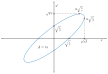
\includegraphics[width=0.8\linewidth,trim={0mm 0mm 0mm 0mm},clip]{figures/Twiss}
    \caption{\label{Fig:Twiss} The phase space ellipse of bunch particles. The figure is recreated from Figure 3.23 by Klauss Wille in \textit{The Physics of Particle Accelerators}~\cite{wille:2001}.}
\end{figure}

% ================================================================================================================================ %
\subsection{Extracting Twiss Parameters from Simulation Data}
\label{Apx:SA:EnTwiss:Sim}

Both OSIRIS and QuickPIC dump the macro particles as large arrays of six-dimensional data, providing each particle's position and momentum vector.
To study the collective motion of particles, it is useful to calculate the bunch total emittance in terms of the RMS value or standard deviation of its particles.
Equation~\ref{EQ:EmittFull} can be rewritten in terms of the statistical distributions of its particles such that
\begin{equation}
    \epsilon = \sqrt{\gamma\sigma_{x}^{2} + 2\alpha\sigma_{x}\sigma_{x^{\prime}} + \beta\sigma_{x^{\prime}}^{2}}, \label{EQ:Emitt}
\end{equation}
where the angle of the $i$-th particles can be taken from its momentum
\begin{equation}
    x_{i}^{\prime} = \frac{p_{i,x}}{p_{i,z}}.
\end{equation}

For a set of macro particles, the emittance can be calculated directly by taking the covariance matrix of the $x$ and $x^{\prime}$ vectors
\begin{equation}
    \mathbf{T} = \mathrm{cov}\left(\mathbf{x}, \mathbf{x}^{\prime}\right), \label{EQ:ECalc1}
\end{equation}
and then taking the square root of its determinant
\begin{equation}
    \epsilon = \sqrt{\mathrm{det}\left(\mathbf{T}\right)}. \label{EQ:ECalc2}
\end{equation}
The Twiss parameters can be extracted from the matrix $\mathbf{T}$ as well:
\begin{equation}
    \alpha = \mathrm{T}_{12}/\epsilon, \quad
    \beta  = \mathrm{T}_{11}/\epsilon, \quad
    \gamma = \mathrm{T}_{22}/\epsilon
\end{equation}

% ================================================================================================================================ %
\section{A Measure for Beam Quality}
\label{Apx:SA:QTilde}

For the emittance study in Publication~\ref{Pub:BL17}, it was necessary to define a convenient unit for the quality of the accelerated bunch in terms of emittance evolution in regions along the bunch length.
In the quasi-linear plus non-linear regime this publication investigates, emittance growth only occurs at the head of the bunch.
However, the region of emittance growth varies when parameters such as charge and beam size changes.
In the study, we defines the quantity
\begin{equation}
    \tilde{Q} = \sum_{m=0}^{M} \frac{1}{N} \left[\sum_{n=0}^{N} Q_{m+n}\right] \cdot \chi(\xi_{m},N),
\end{equation}
where $M$ is the number of longitudinal grid slices of length $\Delta\xi$ which contains macro particles for the witness bunch, and with corresponding coordinate $\xi_{m}$; $N$ is the number of such slices to average over; and $\chi(\xi_{m},N)$ is the step function
\begin{equation}
    \chi(\zeta,N) =
    \begin{cases}
        0, & \frac{\epsilon(\zeta) - \epsilon_{0}}{\epsilon_{0}} > 5\% \\
        1, & \frac{\epsilon(\zeta) - \epsilon_{0}}{\epsilon_{0}} \leq 5\%
    \end{cases}
    \quad\mathrm{for}\quad
    \xi_{m} < \zeta \leq \xi_{m} + N\Delta\xi,
\end{equation}
where $\epsilon(\zeta)$ is the emittance as defined by Equations~\ref{EQ:ECalc1} and~\ref{EQ:ECalc2} for a set of macro particles within the interval $\xi_{m}$ to $\xi_{m} + N\Delta\xi$.
For the studies included in Publication~\ref{Pub:BL17},
\begin{equation}
    M = \left\lfloor \frac{10\sigma_{z}}{\Delta\xi} \right\rceil, \quad
    N = 4.
\end{equation}
The first slice
\begin{equation}
    \xi_{0} = \mu_{\mathrm{eb}} - 5\sigma_{z,\mathrm{eb}} - 0.5\Delta\xi,
\end{equation}
where $\mu_{\mathrm{eb}}$ is the longitudinal centre of the bunch.

\paragraph{Note:} This method may yield a misleading result if the Twiss parameter $\alpha$ varies too much along the length of the bunch.
That is, the emittance can be locally small, and qualify for the $5\%$ criterion, even if the total emittance of the region included in $\tilde{Q}$ is not.
This can easily be checked after the seemingly optimal region of the bunch is known by verifying that its total emittance does not exceed the same criterion.

% ================================================================================================================================ %

    %
%  Appendix : Data Analysis Tools
% ================================
%

\chapter{Data Analysis Tools}
\label{Apx:DA}

The simulation codes used in these studies produce large amounts of data.
It has been very useful to develop a tool for effective analysis of both input and output files.
Most of the initial studies were done using OSIRIS 3 (for Publication \ref{Pub:IPAC15} and \ref{Pub:NAPAC16}), and the final emittance study was done using QuickPIC (Publication \ref{Pub:BL17}).

The analysis tools written for these studies are publicly available on GitHub.
The toolbox for OSIRIS 3 is named OsirisAnalysis \cite{code:osiris_analysis:2013}, and the corresponding toolbox for QuickPIC is named QuickPICAnalysis \cite{code:quickpic_analysis:2017}.
Both toolboxes are written for MATLAB.

This appendix briefly outlines the structure and basic function of these tools.

% Also describe briefly how various beam parameters are calculated.
% This should cover Twiss, and the beam quality number used for the last paper.

% ================================================================================================================================ %
\section{The Osiris Analysis Toolbox}
\label{Tools:OA}

The OsirisAnalysis toolbox is a modular and object oriented data analysis toolbox written in MATLAB.
It was designed as a three layer tool to wrap a single data set of OSIRIS simulation data:

\begin{description}
    \item[Layer 1] consists of the core data wrapper class \emph{OsirisData} with its subclass \emph{OsirisConfig}.
        The \emph{OsirisData} class provides an interface for accessing the raw data files, while the \emph{OsirisConfig} class parses the simulation input file.
        \emph{OsirisData} provides a uniform set of calls for extracting the data, and gives through \emph{OsirisConfig} access to all the simulation parameters and conversion factors for converting OSIRS' normalised units into SI units.
    \item[Layer 2] consists of a set of classes that takes an \emph{OsirisData} object as input, and returns standardised structs of data that can be scaled and converted to preferred units.
    They perform often needed tools and methods to parse data and extract more detailed information from the larger raw datasets.
    \item[Layer 3] consist of a number of useful standardised plots, and a GUI tool to quickly do a preliminary analysis of simulation data.
\end{description}

The idea behind this layering of the analysis tool is to allow the user to choose how many of these they will use.
Only using the first layer will give the user access to all the simulation parameters as well as a method to extract data in a standardised manner, and return a simple matrix of its content.
Adding the second layer gives additional access to automatic unit conversion and other data conversion tools like slicing and line-outs, as well as various properties extracted from the macro particle arrays.
The third layer provides a quick way to browse through the datasets and display density plots, phase space plots, Twiss parameters, time evolution, etc.

% ================================================================================================================================ %
\subsection{Core Objects}
\label{Tools:OALay1}

The innermost layer consists of two classes:

\begin{description}
    \item[OsirisData:] This class wraps the simulation data folder and is the core interface through which data is extracted.
    The class also provides some simple methods for extracting information about the dataset like physical dimensions of the beam and the distribution of the plasma.
    
    \item[OsirisConfig:] This class is a wrapper for the input file itself, and contains a parser for this file which extracts all the relevant information for both analysis and provides lists of available diagnostics for the graphical user interface (GUI).
    All conversion factors to SI units are calculated on the fly when the input file is loaded.
    The \emph{OsirisConfig} class is not intended to be called by the user, but is found as a child object of the \emph{OsirisData} data object.
\end{description}

% ================================================================================================================================ %
\subsection{Data Types}
\label{Tools:OALay2}

The secondary layer of the OsirisAnalysis framework is a set of subclasses under a parent class named \emph{OsirisType}.
The subclasses will give access to specific types of data more or less directly related to the diagnostics types produced by the OSIRIS simulation code.

The classes provided are:

\begin{description}
    \item[Density and Field:] These are classes that produce grid diagnostics data for the particle density data dumps or the field diagnostics data.
    They support all the different density diagnostics outputs of OSIRIS, and will in addition calculate the wakefields from the magnetic and electric fields given by $W = F/q = E - v \times B$.
    \item[Momentum:] This class consists of a set of methods that will calculate the evolution of the beams energy and momentum over several time dumps.
    \item[Phase:] This class provides several tools for phase space diagnostics, including calculations of Twiss parameters.
    \item[UDist:] This class is similar to the \emph{Density} and \emph{Field} classes, and provides methods to process velocity and thermal distribution data.
    \item[Species:] This class provides a few additional specialised tools for calculating energy deposition and gain into and from the plasma by the beams, and is also the class where particle tracking data is parsed.
\end{description}

In addition to these data parsing classes, there is also a \emph{Variables} class that will translate OSIRIS diagnostics variables into readable forms, and into strings usable for plot labels.
There is also a \emph{MathFunc} class that provides a math parser that emulates the one used by OSIRIS to parse mathematical functions from the input files.
This class is mainly used to extract geometric information about beam density based on the function provided in the input file without the need to first run the code to provide raw particle data.

% ================================================================================================================================ %
\subsection{Graphical Interface and Plots}
\label{Tools:OALay3}

The final layer of the OsirisAnalysis framework is a set of very flexible plotting tools.
Most of these have a long list of optional input argument that will change the way data is aggregated and presented.
To make these plots easier to use, most of these optional arguments are available through a graphical interface, also written in MATLAB, named \emph{AnalysisGUI}.

\begin{figure}[hbt]
    \centering
    \includegraphics[width=0.99\linewidth,trim={0mm 0mm 0mm 0mm},clip]{images/OsirisAnalysisGUI}
    \caption{\label{Fig:OAGUI} A screenshot of the OsirisAnalysis GUI tool.}
\end{figure}

% ================================================================================================================================ %
\section{QuickPIC Analysis Framework}
\label{Tools:QA}

The toolbox developed for OSIRIS was also partially rewritten to work with QuickPIC simulations.
As QuickPIC uses more or less the same normalised units, the code required little modification to work with these output files.
The conversion was also made easier by QuickPIC having a simpler and more consistent set out output files and formats.

As QuickPIC was only used for the final set of studies, only the core objects and input file wrapper classes, and the data type classes were converted.
No graphical user Interface was developed for this toolbox, and only a few standardised plots were added.
The analysis toolbox is available on GitHub \cite{code:quickpic_analysis:2017}.


% Back Matters

\backmatter

% Revert to standard italics for Bibliography
\renewcommand{\emph}[1]{\textit{#1}}

\bookmarksetup{startatroot}
\cleardoublepage
\phantomsection
\addcontentsline{toc}{chapter}{Bibliography}
\bibliography{Bibliography,Additional}
\null

\phantomsection
\bookmarksetup{startatroot}
\pdfbookmark{End}{EndOfDoc}
\vspace*{\fill}
\footnotesize
\noindent Document compiled on \today~at~\currenttime
\newline
\pdftexbanner
\cleardoublepage

\end{document}

% ================================================================================================================================ %
